\chapter*{Synthèse en français}
\addcontentsline{toc}{chapter}{Synthèse en français}

\section*{Introduction}
\markboth{Synthèse en français}{Introduction}
\addcontentsline{toc}{section}{Introduction}
La compréhension de la physique des hautes énergies à notre époque repose sur les succès de ses approches théoriques et expérimentales, réalisés dans la seconde moitié du XXe et au début du XXIe siècles. Cette thèse porte sur l'étude expérimentale des propriétés d'une particule fondamentale appelée boson W et sur l'amélioration des techniques expérimentales utilisées dans l'expérience ATLAS. 
\subsection*{Le Modèle Standard de la physique des particules}
\addcontentsline{toc}{subsection}{Le Modèle Standard de la physique des particules}
Le Modèle Standard (MS) de la physique des particules est une théorie quantique des champs développée dans les années 1960-1970 qui décrit la structure et les interactions de la matière au niveau fondamental. Cette théorie postule l'existence de 12 fermions élémentaires et fournit une description de leurs interactions à travers 3 des 4 forces fondamentales connues: électromagnétique, faible et forte. Les médiateurs de ces forces fondamentales sont également décrits comme des particules élémentaires (voir Fig. \ref{fig::SMwiki_synthese}). Les prédictions du Modèle Standard dépendent de 18 paramètres qui doivent être mesurés expérimentalement.

Les bosons W et Z sont les porteurs de l'interactions faible. Le boson W a été découvert expérimentalement en 1983 au CERN, et les mesures de précision de sa masse et de ses propriétés se poursuivent depuis lors. Le boson W étant l'une des pierres angulaires du Modèle Standard, les mesures expérimentales de précision de ses propriétés permettent de tester et d'améliorer les prédictions théoriques. Ceci est la motivation principale de cette thèse.

\begin{figure}[htpb]
	\centering
	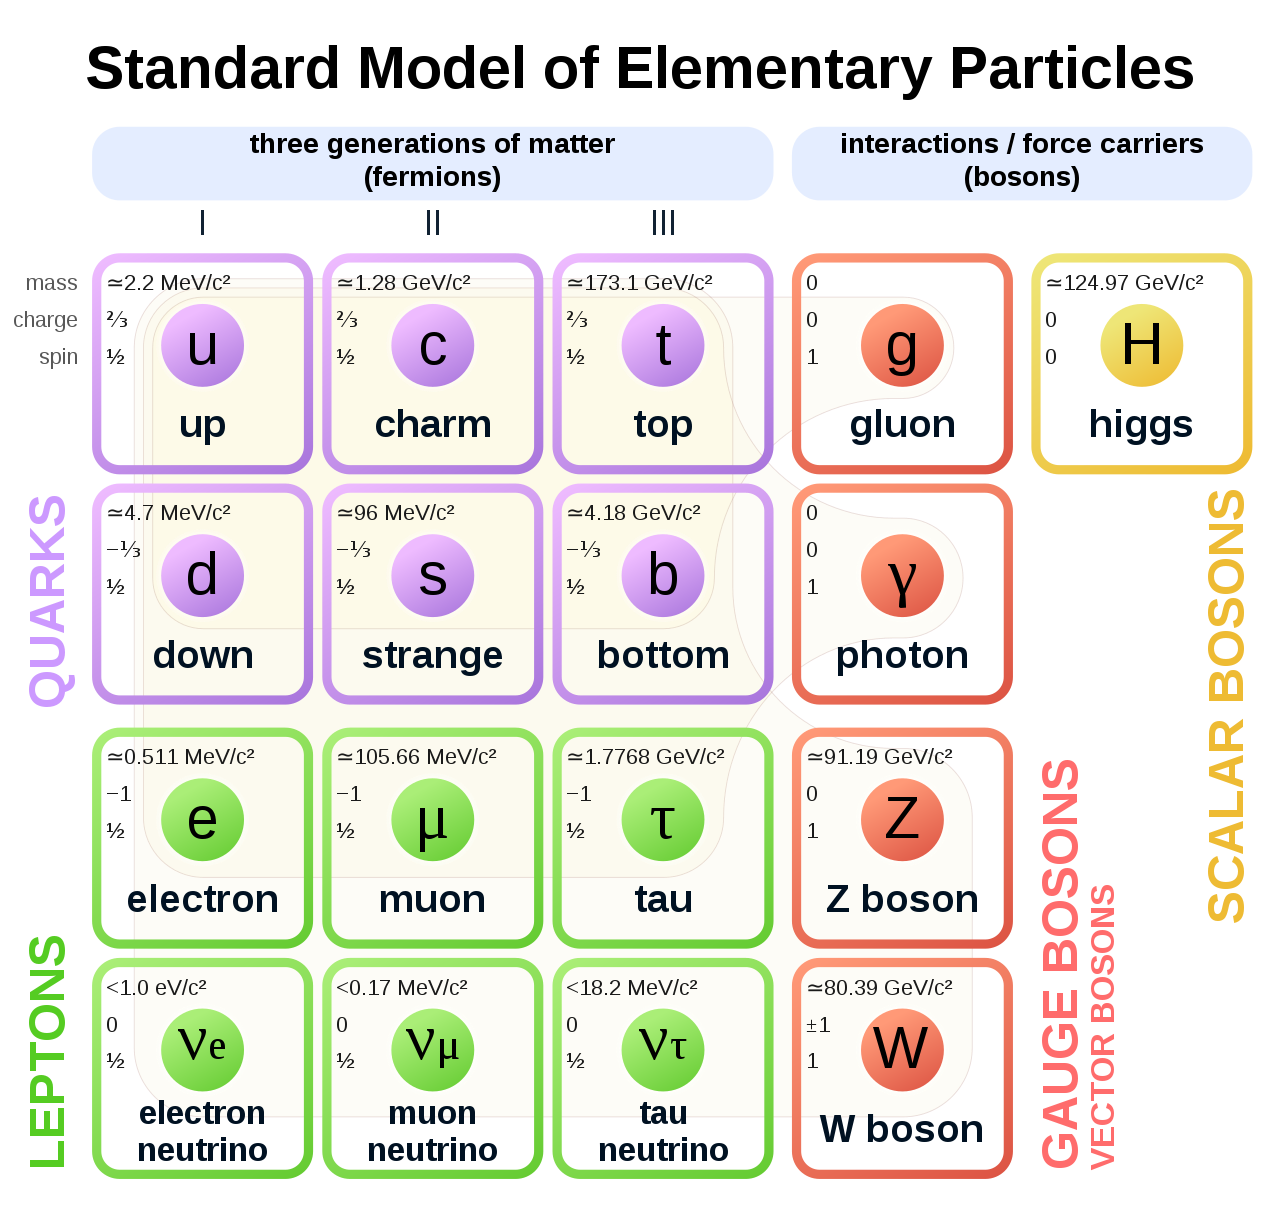
\includegraphics[width=0.7\textwidth,keepaspectratio]{SMwiki.png}
	\caption{Liste des particules du \gls{sm}. }
	\label{fig::SMwiki_synthese}
\end{figure}

\subsection*{Le Grand Collisionneur de Hadrons (LHC) et l’expérience ATLAS}
\addcontentsline{toc}{subsection}{Le Grand Collisionneur de Hadrons (LHC) et l’expérience ATLAS}

Le \gls{lhc} est un accélérateur de particules construit près de la ville de Genève en Suisse. Avec une circonférence de 27 km, c'est le plus grand accélérateur de particules au monde. Il est capable d'accélérer des protons jusqu'à une énergie de 6,5 TeV par particule et des ions de plomb jusqu'à 2,76 TeV par nucléon. Au cours de la deuxième phase, le LHC a délivré des faisceaux collimatés en 4 points d'interaction, à un taux de 40 millions de croisements de paquets par seconde. Les quatre points d'interaction correspondent à quatre expériences basées au LHC: ATLAS, CMS, LHCb et ALICE.

L'expérience ATLAS est un détecteur de particules généraliste de forme cylindrique, de 44 m de long et de 25 m de haut. Il a une structure en forme d'oignon combinant différents types de détecteurs pour permettre une reconstruction des particules la plus efficace possible (voir Fig.\ref{fig::atlas_layout_s}). Après la collision des protons au point d'interaction, les particules générées pénètrent dans le détecteur interne, qui fournit des informations sur la direction, l'impulsion et la charge des particules chargées. Ensuite, les particules atteignent le calorimètre, qui est utilisé pour reconstruire l'énergie et l'impulsion des particules neutres et chargées. Enfin, les particules capables de pénétrer dans le calorimètre atteignent les chambres à muons qui constituent le système de détection le plus à l'extérieur du calorimètre ATLAS. Les chambres à muons sont utilisées pour reconstruire la direction, l'impulsion et la charge des muons.
\begin{figure}[htpb]
	\centering
	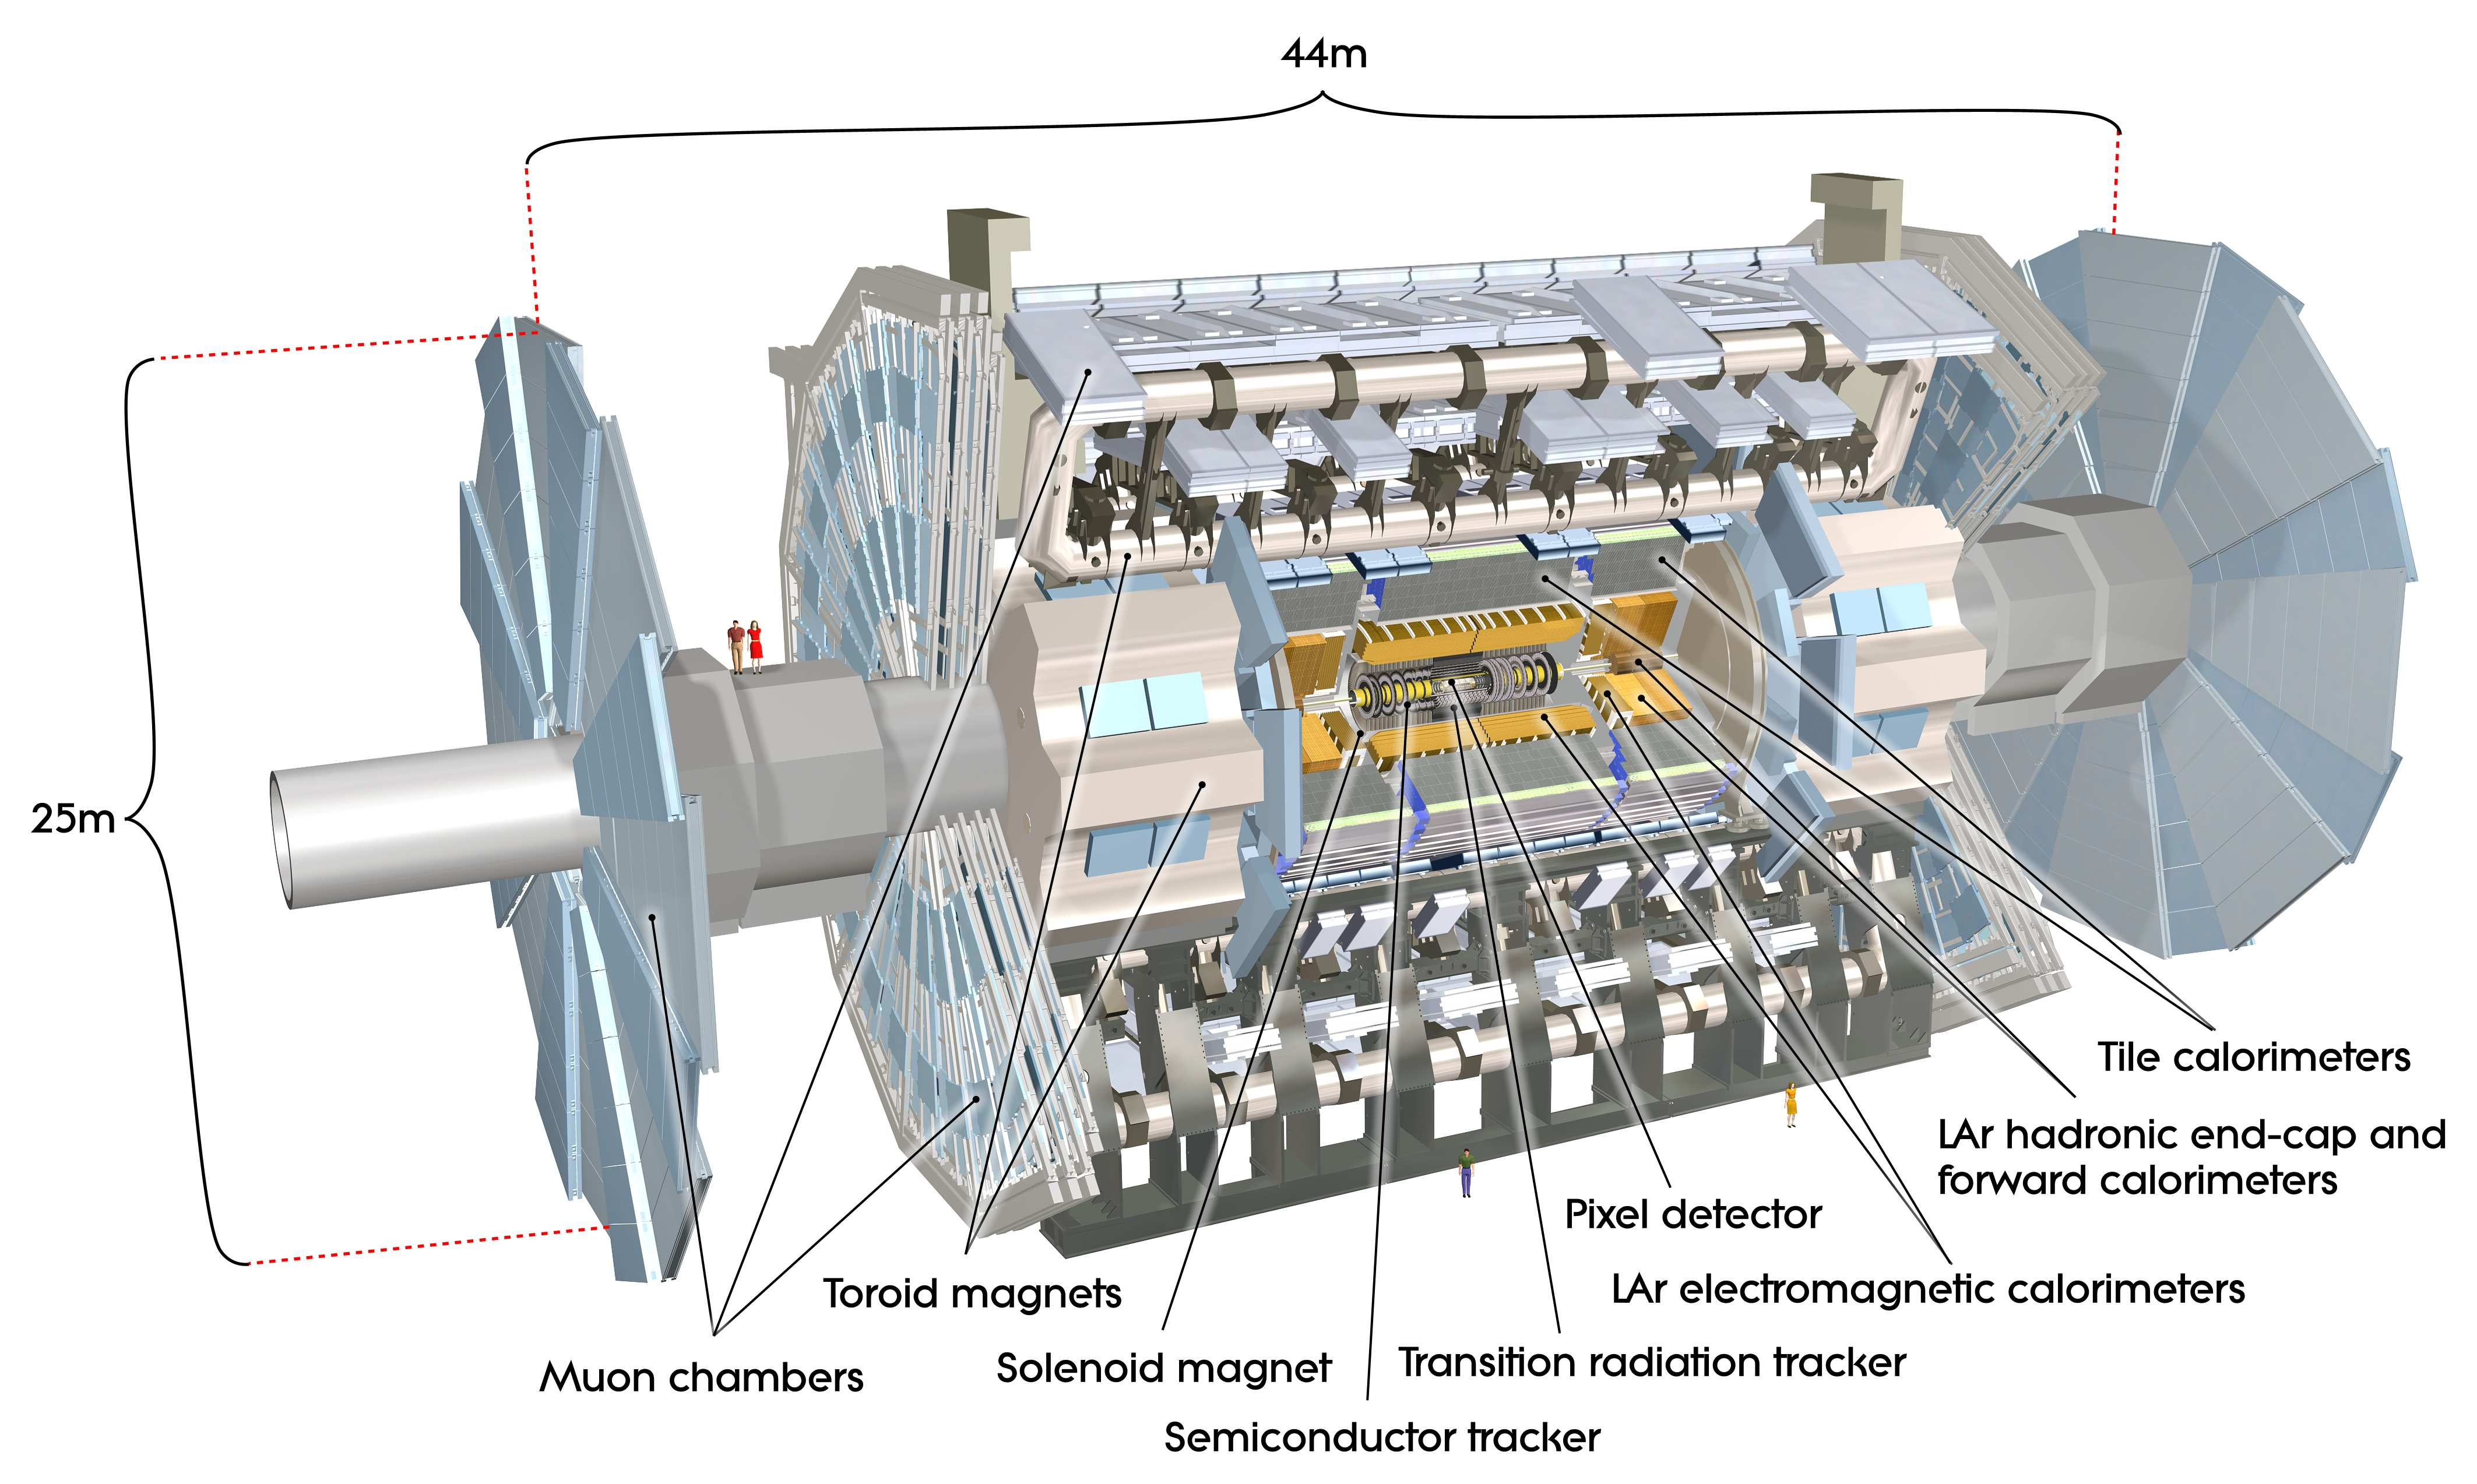
\includegraphics[width=0.7\textwidth,keepaspectratio]{image--001.jpg}
	\caption{ Schéma du détecteur ATLAS.}
	\label{fig::atlas_layout_s}
\end{figure}

\section*{Correction des formes des cascades électromagnétiques}
\markboth{Synthèse en français}{Correction des formes des cascades électromagnétique}
\addcontentsline{toc}{section}{Correction des formes des cascades électromagnétiques}
Le calorimètre électromagnétique, \gls{emc}, est conçu pour reconstruire l'énergie des électrons et des photons qui atteignent le calorimètre. Les informations de l'\gls{emc} sont également utilisées pour l'identification des particules et le rejet du bruit de fond.

\begin{figure}[htpb]
	\centering
	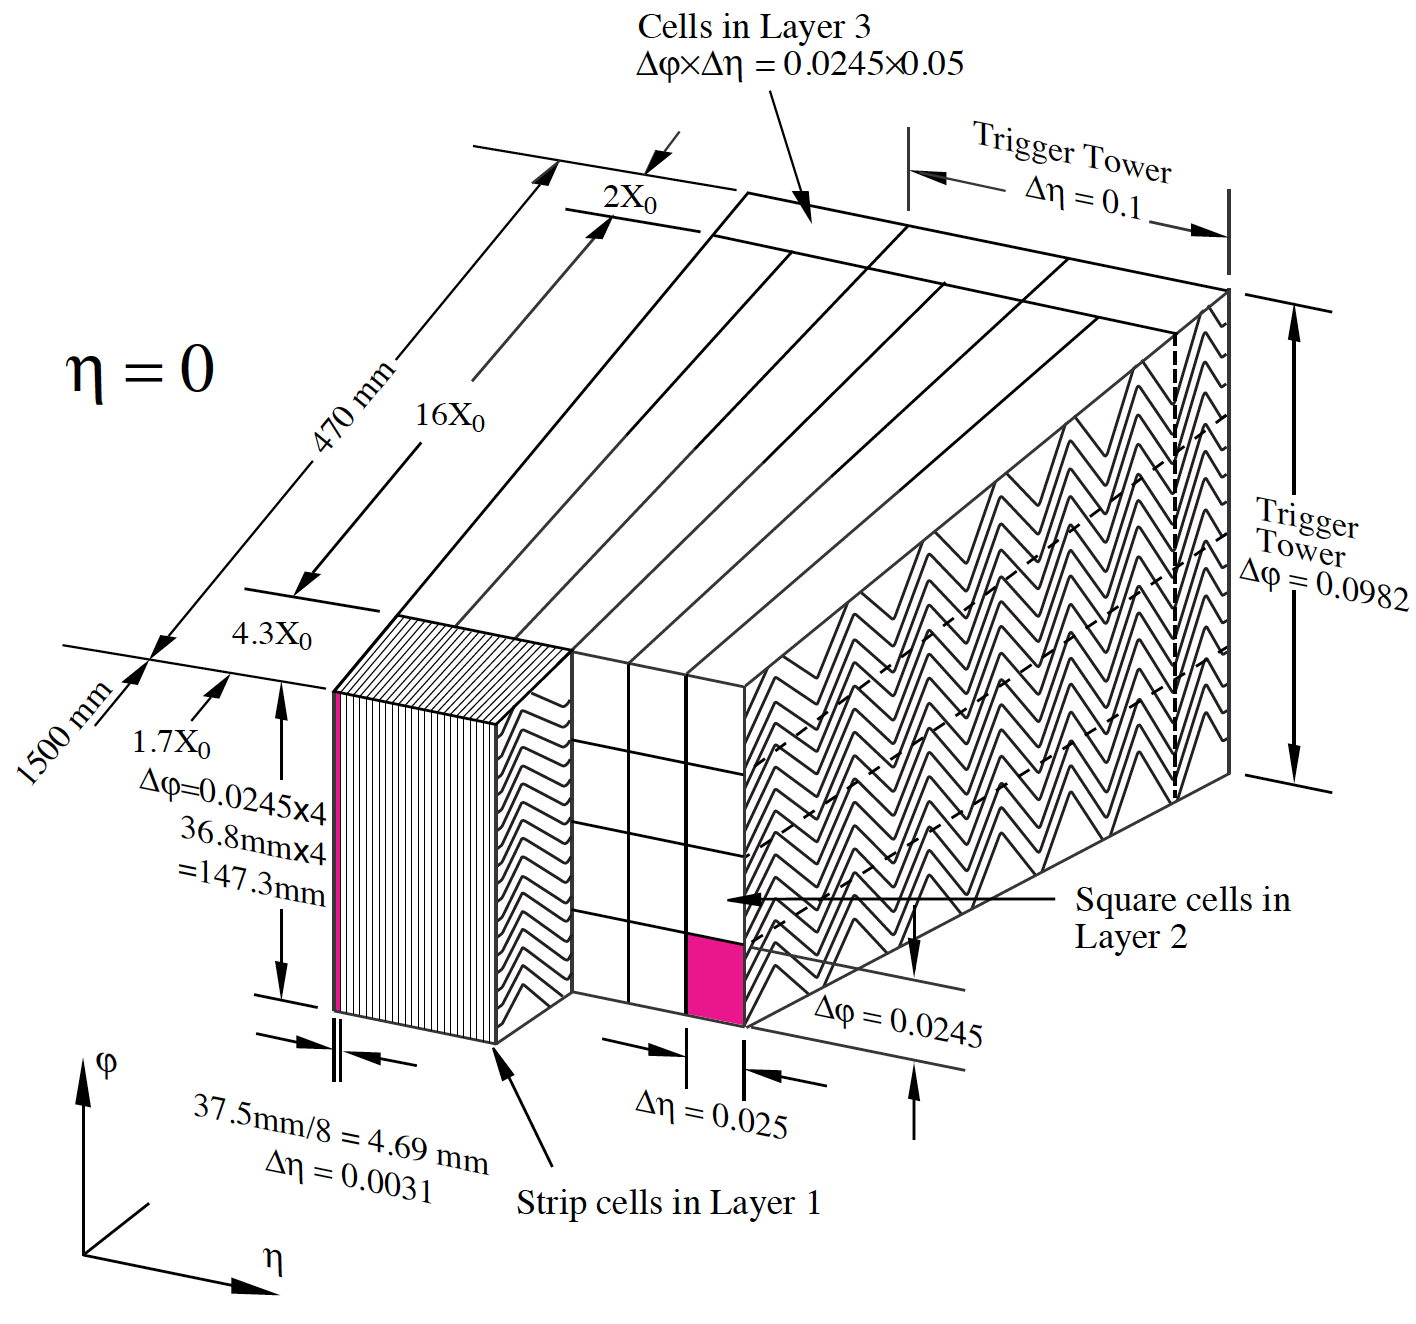
\includegraphics[width=0.7\textwidth,keepaspectratio]{EMcalo_layers.png}
	\caption{ Couches du calorimètre électromagnétique d'ATLAS.}
	\label{fig::calorimeter_layers_s}
\end{figure}

L'\gls{emc} se compose de trois couches et d'un pré-échantillonneur (voir Fig. \ref{fig::calorimeter_layers_s}). La deuxième couche est la plus épaisse, elle absorbe l'essentiel de l'énergie des électrons et des photons. La deuxième couche a une granularité fine dans les deux dimensions $\eta$ et $\phi$, et fournit des informations sur le développement transverse de la cascade électromagnétique. Ces informations sont utilisées pour calculer un certain nombre d'observables appelées formes de la cascade, puis utilisées comme paramètres d'entrée pour un algorithme MVA qui prend une décision sur l'identification des particules. Il existe trois formes de cascades qui reflètent le développement de la cascade dans la troisième couche du calorimètre:

\begin{itemize}
	\item La largeur latérale de la cascade $ W_{\ eta 2} = \sqrt{\sum(E_i \eta^{2}_{i}) - (\sum (E_i \eta_{i}) / \sum(E_i))^2} $ calculée dans une fenêtre de 3x5 cellules.
	\item $ R_{\phi} $ - rapport de l'énergie dans les cellules 3x3 sur l'énergie dans les cellules 3x7 centrées autour de la cellule la plus énergétique.
	\item $ R_{\eta} $ - rapport de l'énergie dans les cellules 3x7 sur l'énergie dans les cellules 7x7 centrées autour de la cellule la plus énergétique.
\end{itemize}

Pour des raisons inexpliquées, la modélisation des formes de cascade dans la simulation Monte-Carlo est imparfaite et il y a un écart substantiel avec les données (voir Fig. \ref{fig::sshapes_corrected}). Ces écarts doivent être corrigés avec des facteurs d'étalonnage, à qui sont associées des incertitudes dépendant du $p_T$. Cette thèse présente une méthode basée sur les données pour corriger ces écarts en redistribuant l'énergie entre les cellules des amas calorimétriques.

\begin{figure*}[ht!]
	\subfloat{%
		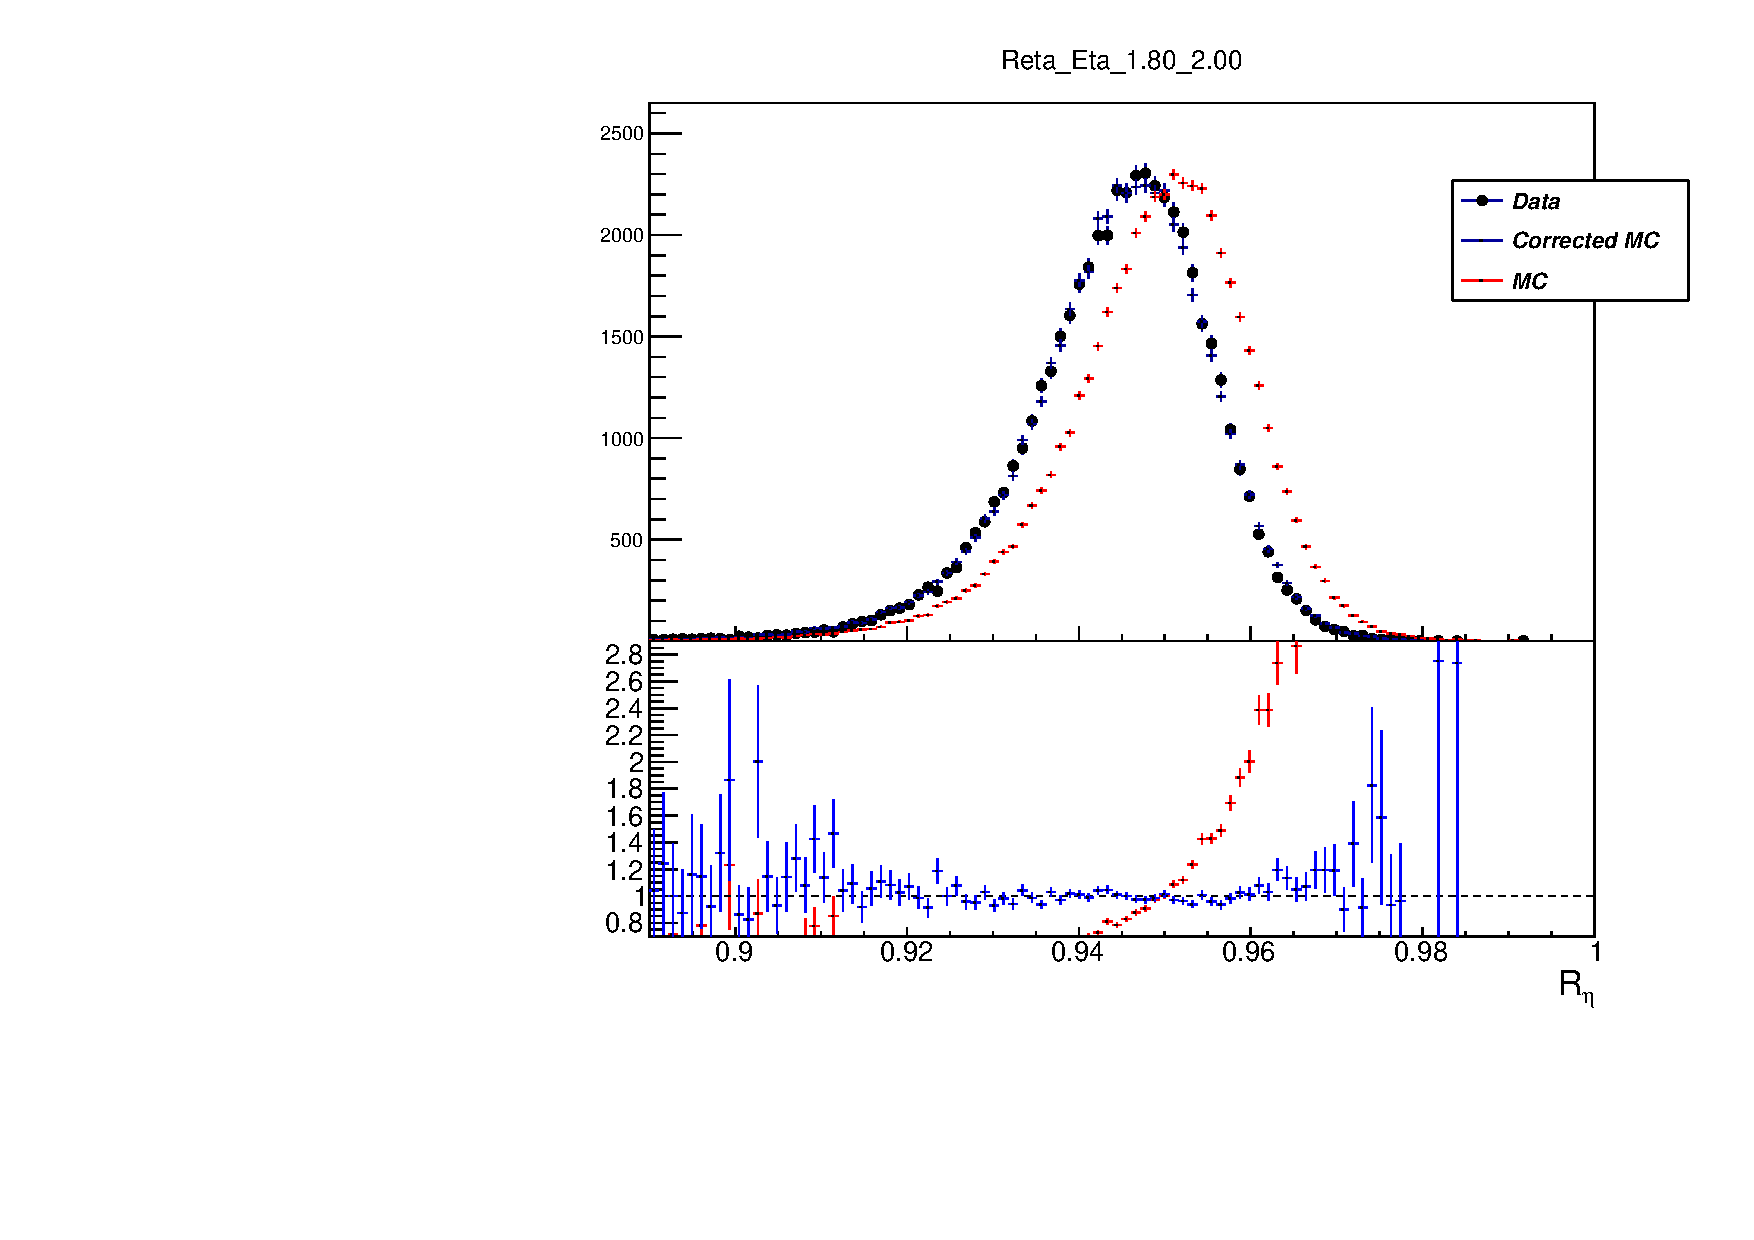
\includegraphics[width=0.33\textwidth]{Reta_Eta_18_20_Athena}}
	\quad
	\subfloat {%
		\includegraphics[width=0.33\textwidth]{weta2_Eta_18_20_Athena}}
	\quad
	\subfloat{%
		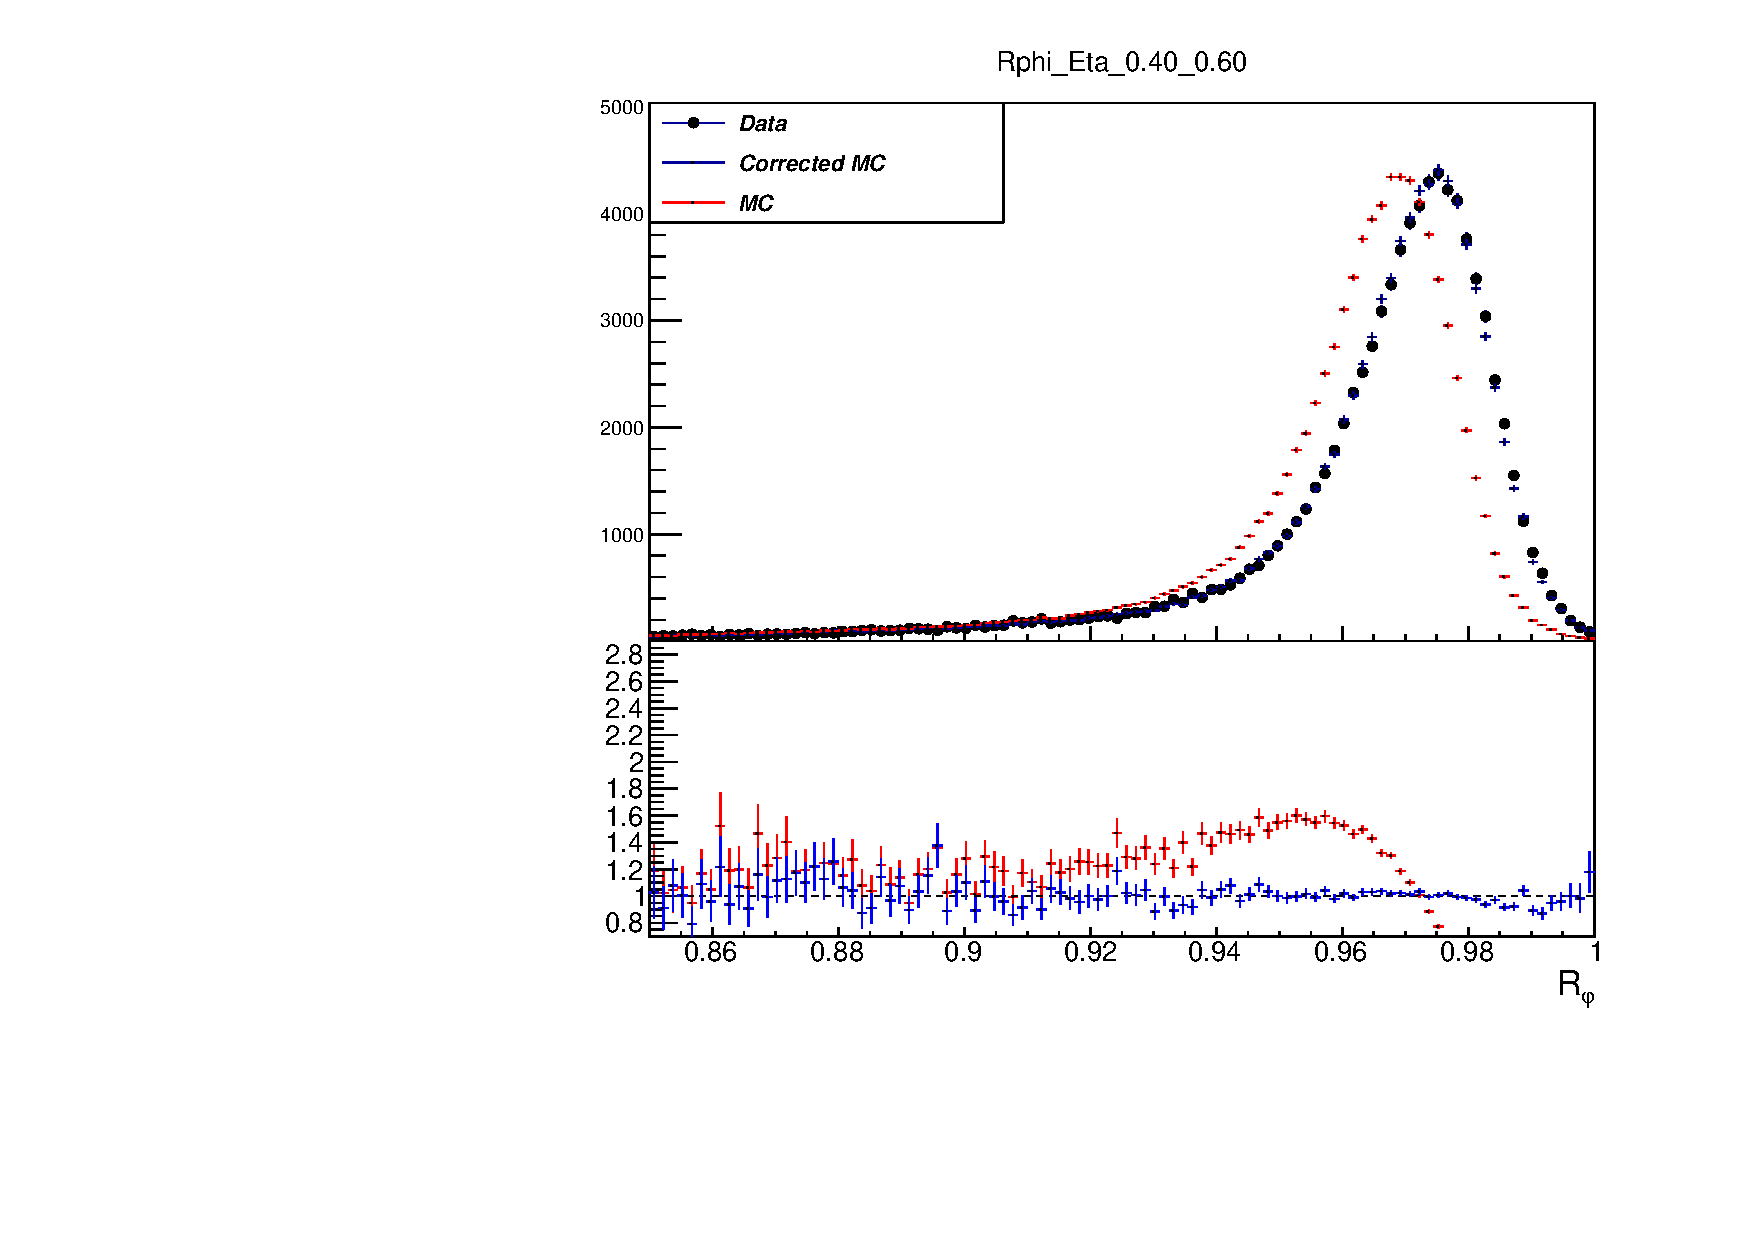
\includegraphics[width=0.33\textwidth]{Rphi_Eta_4_6_Athena}}\\
	\caption{ 	\label{fig::sshapes_corrected} \textbf{Left}: $R_{\eta }$ dans $|\eta| = (1.8,2.0)$. \textbf{Central}: $W_{\eta^2 }$ dans $|\eta| = (1.8,2.0)$. \textbf{Right}: $R_{\phi }$ dans $|\eta| = (0.4,0.6)$.  }
\end{figure*}

Les formes de cascades corrigées dans la simulation sont en bon accord avec les données et se traduisent par un accord significativement meilleur dans les efficacités d'identification (voir Fig. \ref{fig::SF_s}). L'effet de la correction est le plus important dans la région des bouchons où il atteint 3\%. La méthode proposée a été intégrée dans le logiciel de reconstruction officiel de l'expérience ATLAS et sera utilisée par défaut pour les analyses du Run3.
\begin{figure}[htbp]
	\centering
	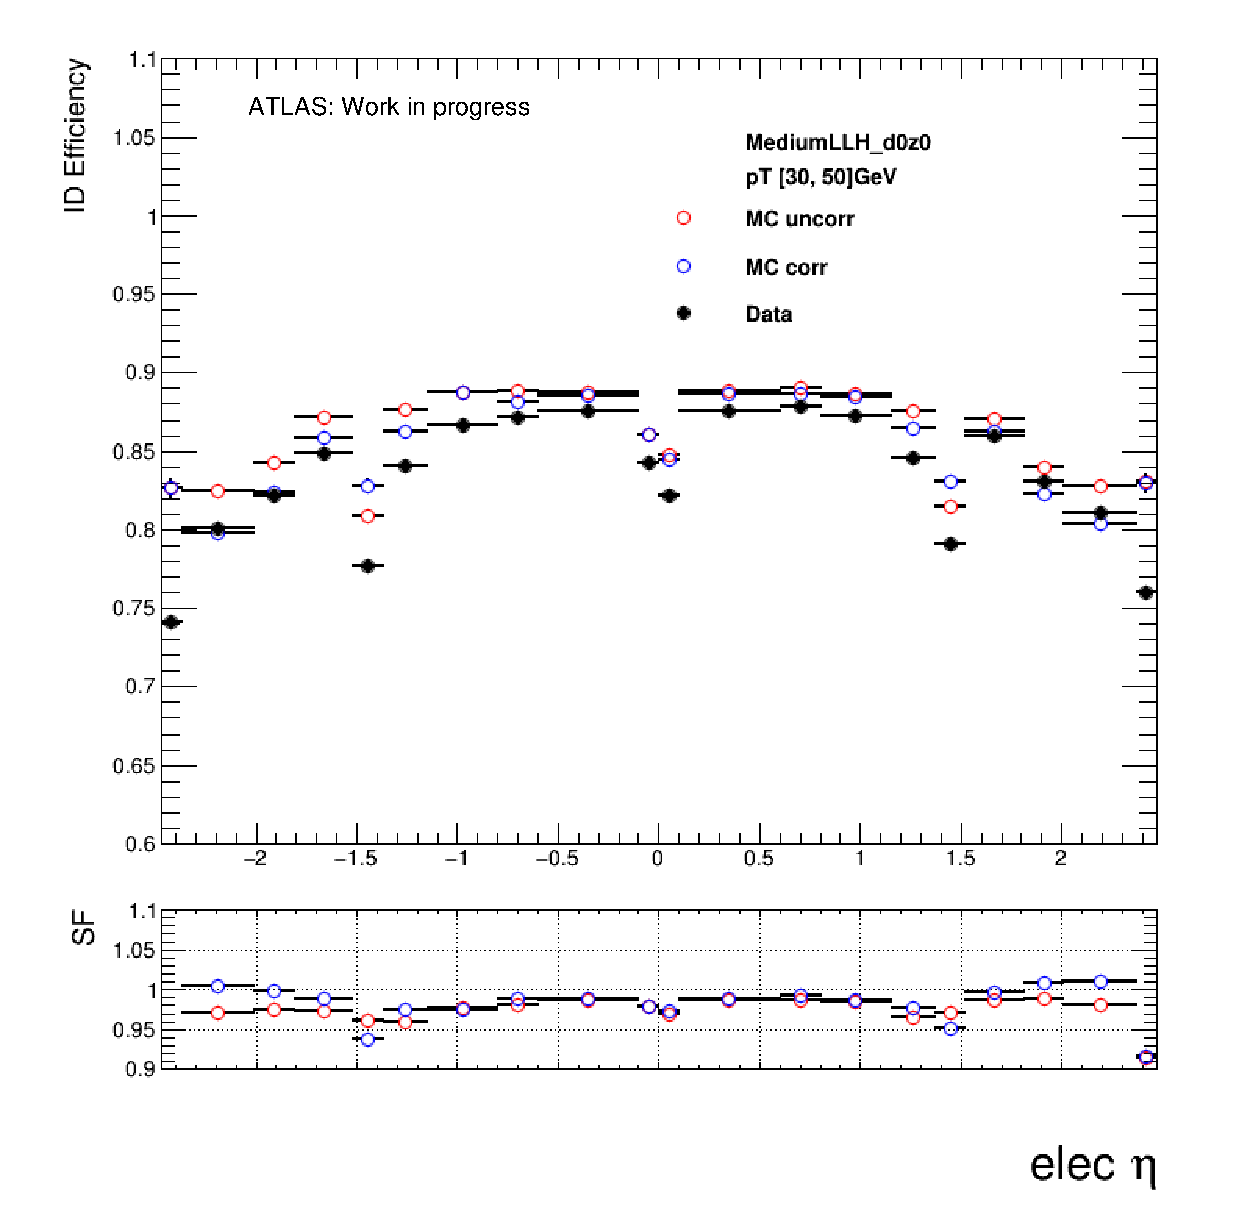
\includegraphics[width=0.7\textwidth,keepaspectratio]{MCeffm247tom237.pdf}\\
	\caption{Efficacité d'identification des électrons en fonction de leur pseudo-rapidité.}
	\label{fig::SF_s}
\end{figure}
\clearpage
\section*{Spectre en impulsion transverse du boson W}
\markboth{Synthèse en français}{Spectre en impulsion transverse du boson W}
\addcontentsline{toc}{section}{Spectre en impulsion transverse du boson W}
La mesure du spectre en impulsion transverse ($p_T$) du boson W est un objectif difficile mais important. À l'ordre dominant (Fig. \ref{fig::w_diagrams_a}), le boson $p_T$ du W est principalement dû aux mouvements intrinsèques du parton et ne dépasse pas 1 GeV. La distribution en impulsion transverse observée, qui atteint des centaines de GeV, est due aux radiations dans l'état initial, qui est un processus survenant à l'ordre suivant, NLO (voir Fig. \ref{fig::w_diagrams_b}). Cela permet de tester les prédictions du Modèle Standard, en comparant la simulation aux données.

\begin{figure}[htbp]
	\begin{subfigure}[t]{0.48\textwidth}
		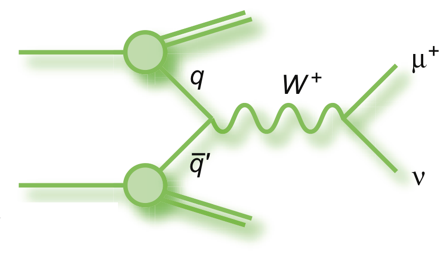
\includegraphics[width=\textwidth,keepaspectratio]{image_2021_02_08T04_22_38_855Z}
		\caption[W production leading order]{Diagramme de Feynman de la production de boson W à l'ordre dominant.}
		\label{fig::w_diagrams_a}
	\end{subfigure}
	\hfill
	\begin{subfigure}[t]{0.48\textwidth}
		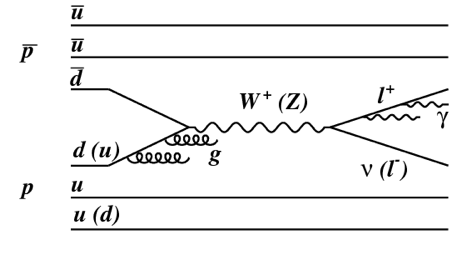
\includegraphics[width=\textwidth,keepaspectratio]{image_2021_02_08T04_22_43_517Z}
		\caption[W production NLO]{Production de boson W à l'ordre NLO.}
		\label{fig::w_diagrams_b}
	\end{subfigure}
\end{figure}


La deuxième motivation vient du fait que la modélisation précise de la distribution en impulsion transverse du W est nécessaire à la mesure précise de la masse du boson W. Étant l'un des paramètres d'entrée du Modèle Standard, la précision de cette mesure a donc des implications sur toutes les prédictions de la théorie. La modélisation théorique du $p_T$ du W est la deuxième incertitude dominante dans la mesure de la masse du boson W réalisée par la collaboration ATLAS.

\begin{figure}[htbp]
	\begin{subfigure}[t]{0.48\textwidth}
		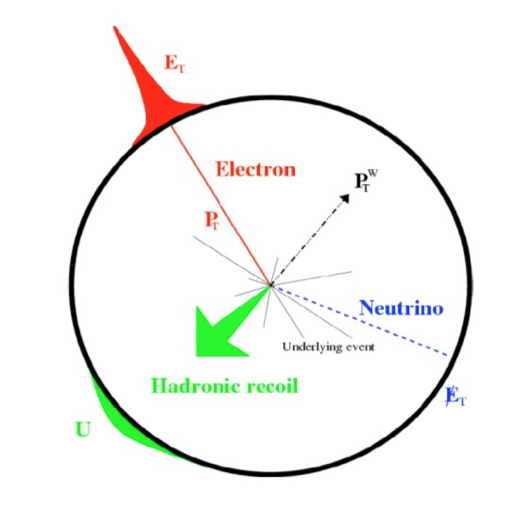
\includegraphics[width=\textwidth,keepaspectratio]{image_2021_02_08T04_22_47_871Z}
		\caption[Hadronic recoil]{Schéma du recul hadronique.}
		\label{fig::hr_s}
	\end{subfigure}
	\hfill
	\begin{subfigure}[t]{0.48\textwidth}
		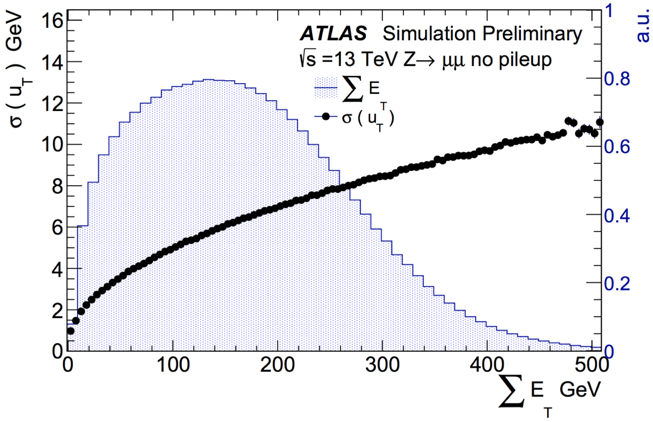
\includegraphics[width=\textwidth,keepaspectratio]{image_2021_02_08T18_35_22_104Z}
		\caption[Pile-up dependence]{Dépendance en empilement du recul hadronique.}
		\label{fig::hr_pileup_s}
	\end{subfigure}
	\label{fig::hr_sss}
	\caption[The hadronic recoil plots]{Le recul hadronique.}
\end{figure}
La mesure de l'impulsion transverse du boson W est difficile. En raison de la présence d'un neutrino dans l'état final, il est impossible de reconstruire le $p_T$ du boson W directement à partir de ses produits de désintégration. C'est pourquoi il est reconstruit en utilisant une observable appelée recul hadronique. Le recul hadronique est supposé refléter la somme des impulsions transverses des radiations dans l'état initial et être égal en magnitude et antiparallèle au $p_T$ du boson W  (voir Fig. \ref{fig::hr_s}). Il est défini pour chaque événement comme la somme vectorielle de tous les \textit{particle flow objects} (PFOs), à l'exclusion des produits de désintégration du boson vecteur. La résolution du recul hadronique dépend directement de l'empilement (Fig. \ref{fig::hr_pileup_s}), ce qui a motivé l'utilisation de données à faible taux d'empilement, collectées par l'expérience ATLAS en 2017 et en 2018.

Bien que le recul hadronique soit très corrélé avec le $p_T$  du boson W, la forme de sa distribution peut être très différente en raison des effets de détecteur. Afin de restaurer la distribution sous-jacente, une procédure appelée déconvolution est utilisée. Après avoir déconvolué le recul hadronique, il devient possible de comparer la distribution obtenue avec les prédictions de la simulation.
\begin{figure}[htbp]
	\begin{subfigure}[t]{0.48\textwidth}
		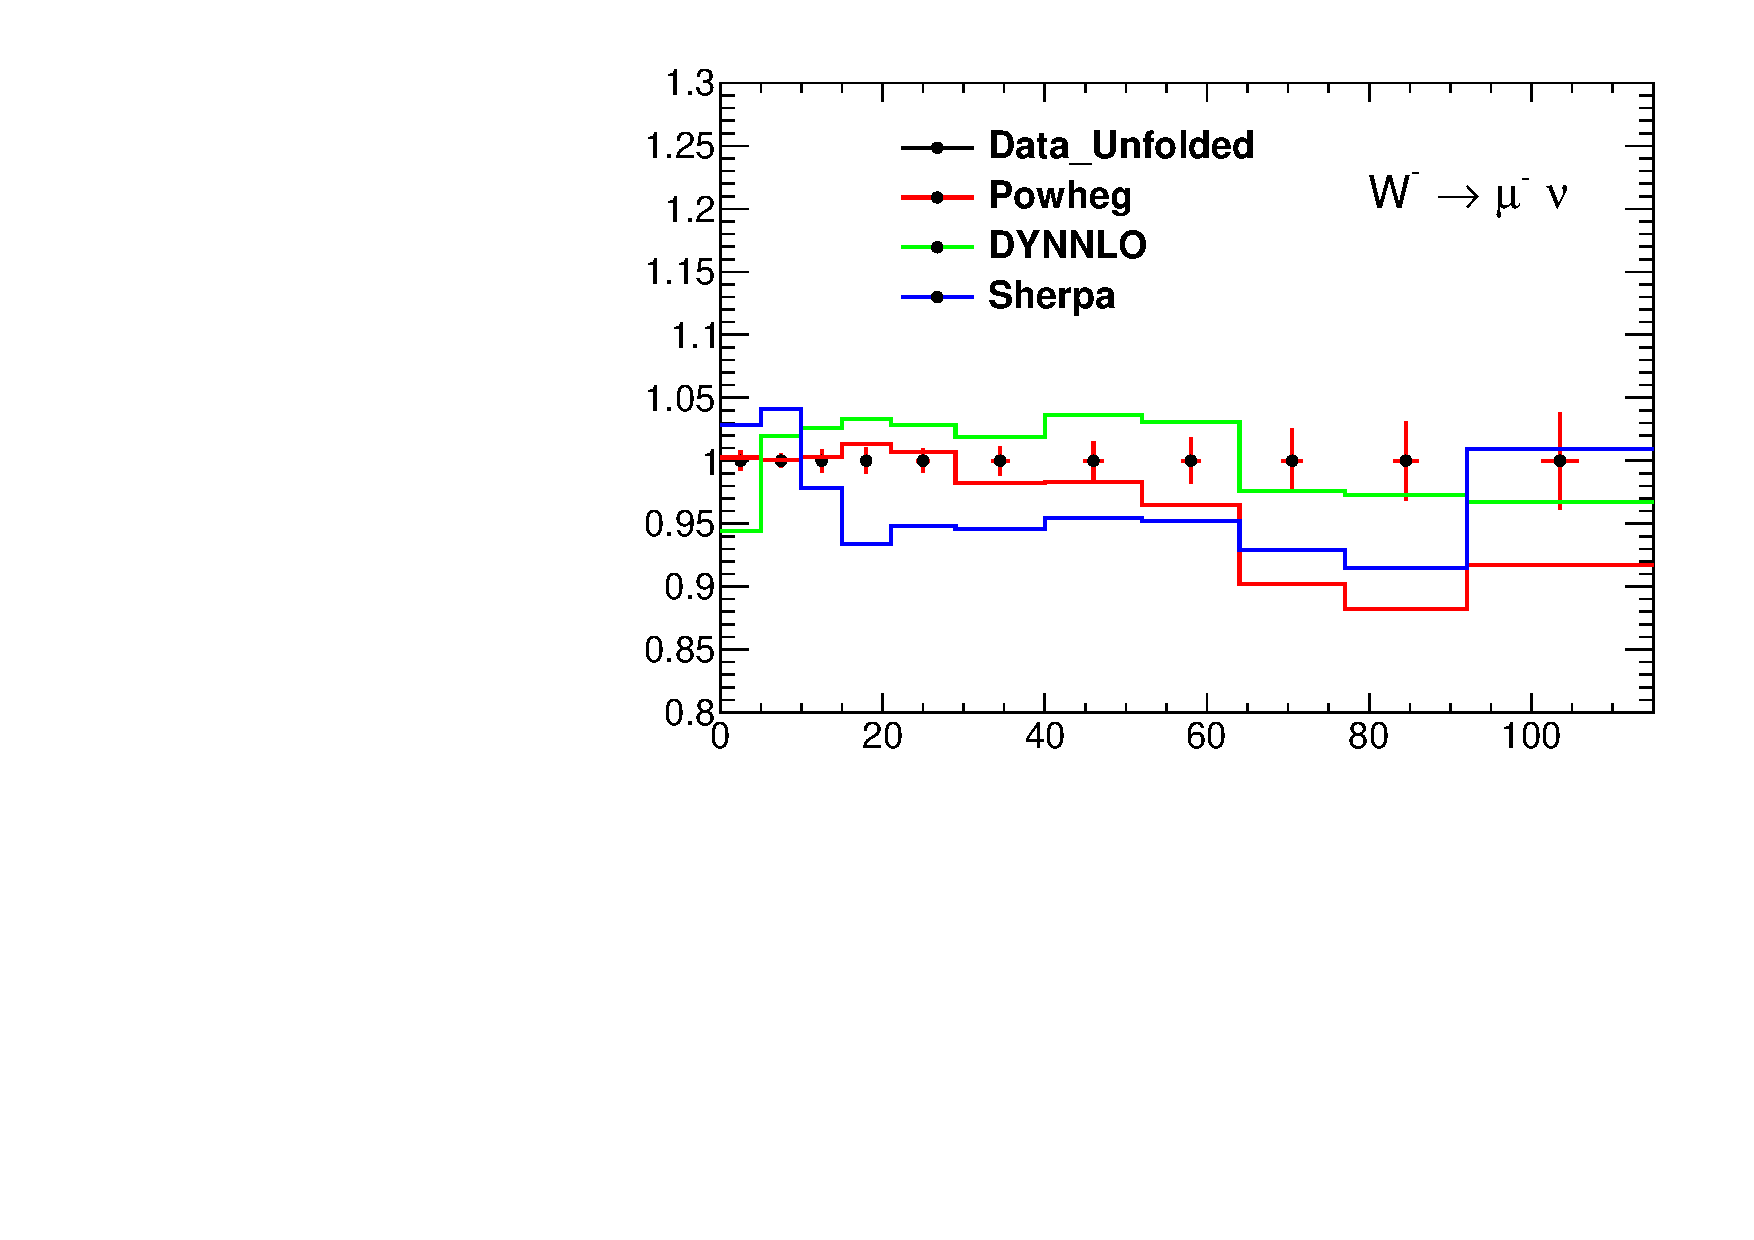
\includegraphics[width=\textwidth,keepaspectratio]{pt_unfolded_Wminusmunu5TeV}
	\end{subfigure}
	\hfill
	\begin{subfigure}[t]{0.48\textwidth}
		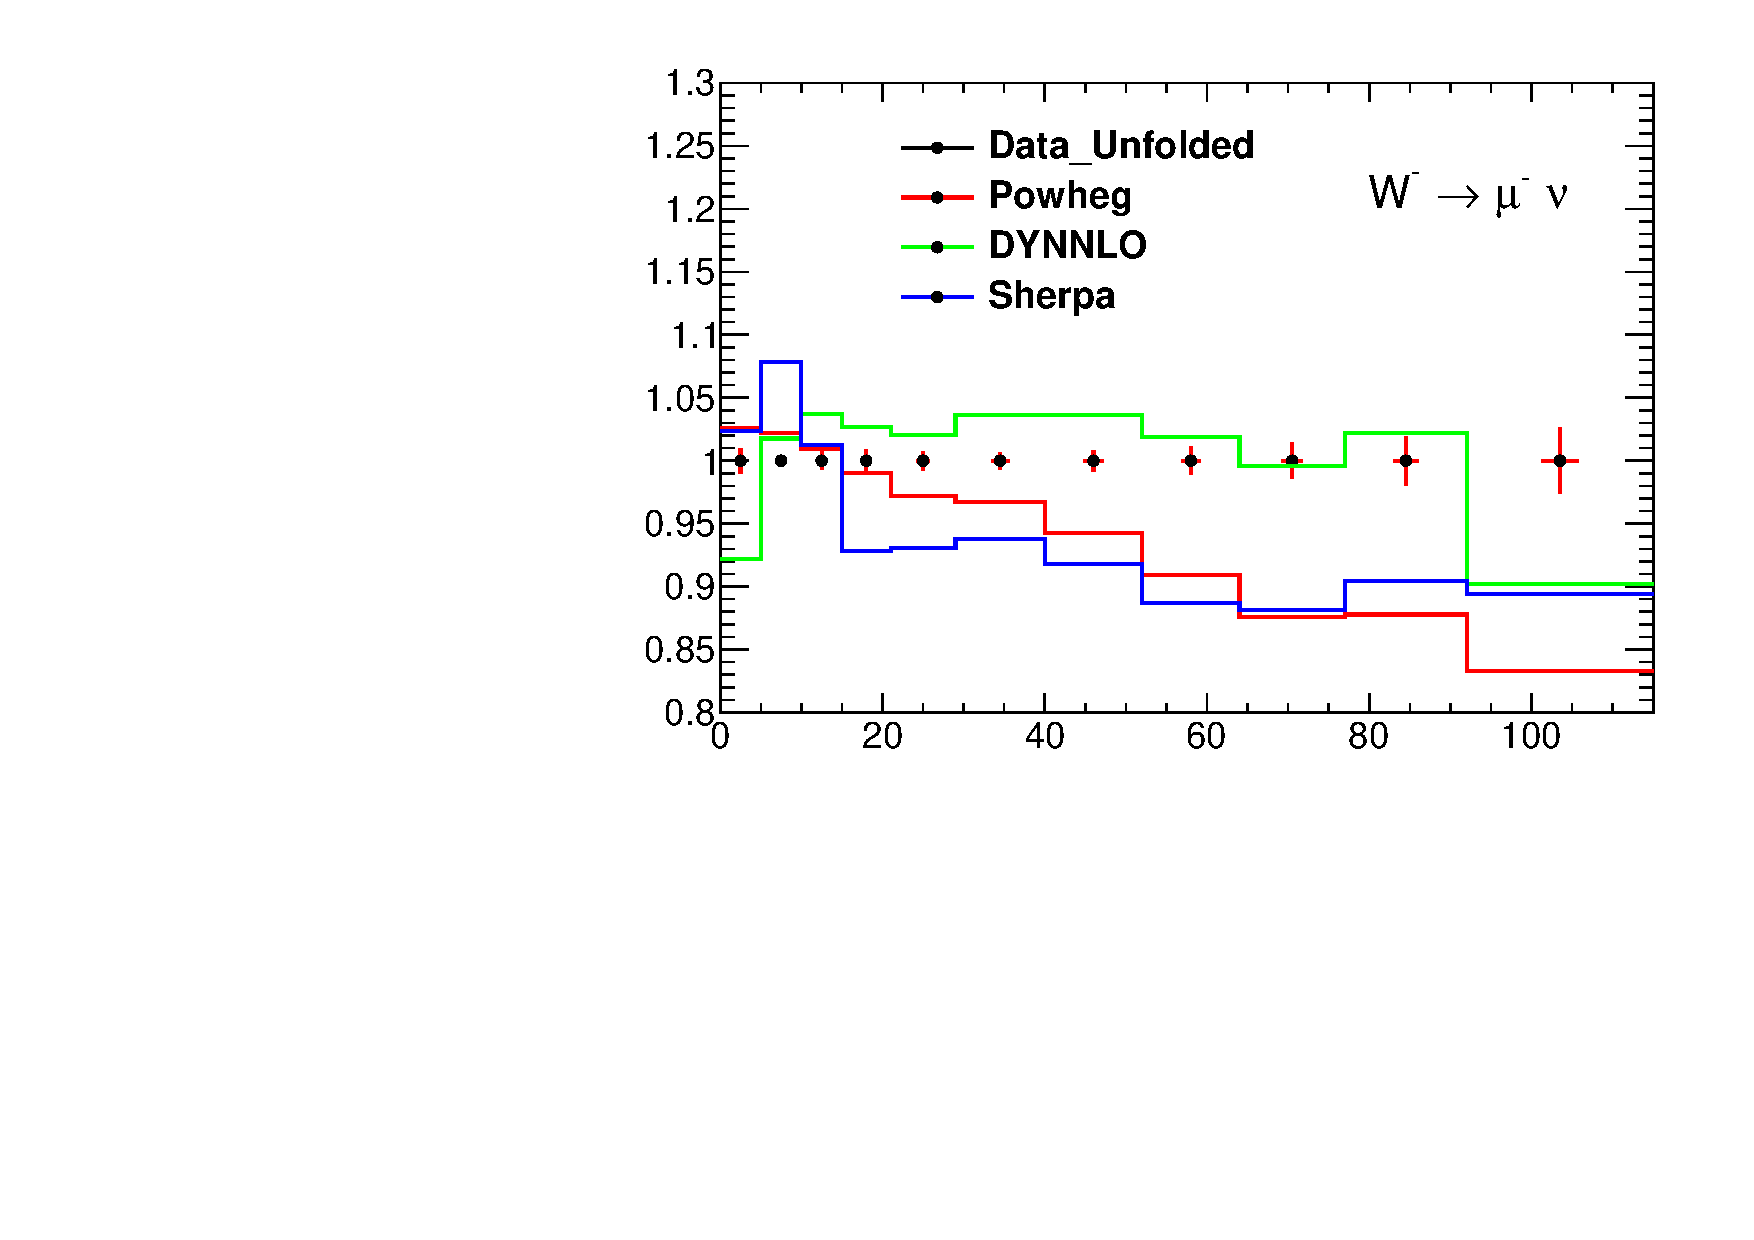
\includegraphics[width=\textwidth,keepaspectratio]{pt_unfolded_Wminusmunu13TeV}
	\end{subfigure}
	\caption[Comparison with MC spectra]{Spectre déconvolué comparé aux modèles théoriques pour le canal $W^{-}\rightarrow \mu^{-} \nu$ à 5 TeV (gauche) et à 13 TeV (droite).}
	\label{fig::spectrum_comparison}
\end{figure}

Il apparait que le spectre mesuré est en relativement bon accord avec les modèles à 5 TeV, tandis qu'à 13 TeV aucun des générateurs MC ne fournit une prédiction compatible.
\section*{Reconstruction du recul hadronique à l'aide de réseaux neuronaux profonds}
\addcontentsline{toc}{section}{Reconstruction du recul hadronique à l'aide de réseaux neuronaux profonds}
\markboth{Synthèse en français}{Reconstruction du recul hadronique à l'aide de réseaux neuronaux profonds}
La résolution de la mesure du recul hadronique est cruciale pour la détermination de la distribution du spectre en $p_T$ du W. Les méthodes modernes d'analyse de données permettent d'améliorer la résolution événement par événement. Afin d'améliorer la résolution, un réseau neuronal profond a été utilisé avec les paramètres suivants:
\begin{itemize}
	\item échantillon d'entrainement : 12 734 109 événements, échantillon de validation: 3 034 130 événements.
	\item Système : Keras / Tensorflow.
	\item Fonction objectif: erreur quadratique moyenne.
	\item Optimiseur: Adam, étape: 0,001.
	\item Taille du lot: 3900 événements.
	\item Trois couches denses cachées de 256 nœuds chacune.
	\item couche de normalisation par lots après chaque couche cachée.
\end{itemize}

\begin{figure}[htbp]
	\begin{subfigure}[t]{0.48\textwidth}
		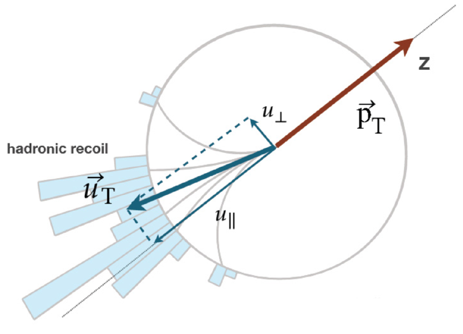
\includegraphics[width=\textwidth,keepaspectratio]{image_2021_02_08T18_21_32_976Z}
		\caption[Bootstrap HR]{Décomposition du recul hadronique.}
		\label{fig::hr_decomp}
	\end{subfigure}
	\hfill
	\begin{subfigure}[t]{0.48\textwidth}
		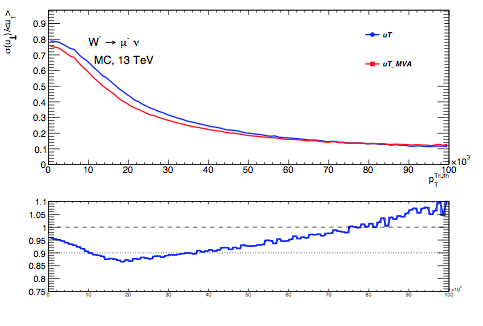
\includegraphics[width=\textwidth,keepaspectratio]{image_2021_02_08T18_20_47_509Z}
		\caption[Bootstrap HR MVA]{Amélioration de la résolution du recul hadronique par le DNN.}
		\label{fig::hr_resolution}
	\end{subfigure}
	\label{fig::hr_ss}
\end{figure}


Cette configuration a été testée pour être la plus efficace possible dans des conditions données. La normalisation par lots a amélioré la stabilité de l'ajustement et réduit le temps d'entraînement d'un facteur cinq environ. La liste suivante des paramètres d'entrée a été utilisée:
\begin {itemize}
\item Le vecteur du recul hadronique $\vec{u_{T}} $.
\item $\vec{u^{chargé}_{T}} $ - la somme vectorielle des $\vec{p_ {T}}$ des PFOs chargés .
\item $\vec{u^{neutre}_{T}} $ - la somme vectorielle des $\vec{p_ {T}}$ des PFOs neutres .
\item $\Sigma E_T$, $\Sigma E^{chargé}_T$, $\Sigma E^ {neutre}_T$ - les sommes scalaires des énergies transverses.
\item Les $p_T$s des deux jets de plus hauts $p_T$s.
\item Le nombre de vertex primaires
\item Le nombre de PFOs chargés et neutres dans l'événement.
\item Les impulsions transverses des cinq PFO neutres et chargés de plus hauts $p_T$s.
\end {itemize}
L'algorithme somme jusqu'à un total de 38 paramètres d'entrée pour la régression des deux composantes du $\vec{p_T}$ du boson W.


\begin{figure}[htbp]
	\begin{subfigure}[t]{0.48\textwidth}
		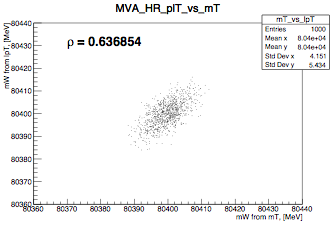
\includegraphics[width=\textwidth,keepaspectratio]{image_2021_02_09T02_14_35_538Z}
		\caption[Bootstrap HR]{Pseudo-expériences pour le recul hadronique nominal.}
		\label{fig::boot}
	\end{subfigure}
	\hfill
	\begin{subfigure}[t]{0.48\textwidth}
		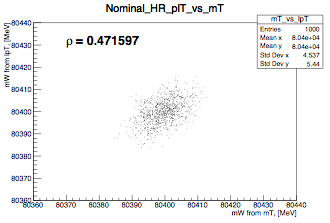
\includegraphics[width=\textwidth,keepaspectratio]{image_2021_02_09T02_14_29_701Z}
		\caption[Bootstrap HR MVA]{Pseudo-expériences pour le recul hadronique reconstruit avec le DNN.}
		\label{fig::boot_mva}
	\end{subfigure}
	\label{fig::nn_s}
\end{figure}

En raison des effets de détecteur, le vecteur du recul hadronique est différent de celui du $p_T$ du boson W en magnitude, et de plus ne lui est pas exactement antiparallèle (voir Fig. \ref{fig::hr_decomp}). La résolution du recul hadronique peut être représentée comme l'étalement de la composante perpendiculaire du recul hadronique $\sigma(u_{\perp})$. La Fig. \ref{fig::hr_resolution} montre environ 10\% d'amélioration provenant de l'utilisation du réseau neuronal profond pour la reconstruction du recul hadronique.

Une résolution de recul hadronique améliorée se traduit également par une meilleure sensibilité des observables à la masse du boson W. Ceci est testé en utilisant 1000 pseudo-expériences et résulte en une plus petite largeur de la masse transverse lorsque le réseau neuronal est utilisé (voir les figures \ref{fig::boot} et \ref{fig::boot_mva}).
\section*{Conclusions}
\markboth{Synthèse en français}{Conclusions}
\addcontentsline{toc}{section}{Conclusions}
Dans cette thèse, trois contributions principales liées à la mesure des propriétés du boson W et aux performances globales du détecteur ATLAS sont présentées.

La correction des formes des cascades dans le calorimètre électromagnétique a permis de corriger l'efficacité d'identification dans la simulation, gagnant 1 à 3\% dans la région des bouchons. L'algorithme développé a été adopté comme défaut pour les prochaines analyses de l'expérience ATLAS durant le Run3.

La mesure de la distribution en impulsion transverse du boson W a permis d'effectuer une comparaison avec les modèles MC existants. La comparaison a révélé un bon accord à 5 TeV, mais un écart significatif à 13 TeV. La précision obtenue permettrait de réduire considérablement l'incertitude de modélisation théorique pour la mesure de la masse du boson W.

L'utilisation d'algorithmes d'apprentissage profond a permis d'améliorer la reconstruction du recul hadronique, permettant une amélioration d'environ 10\% de la résolution dans la région la plus importante de faible impulsion transverse. Elle a également entraîné une sensibilité accrue des observables à la masse du boson W, qui a été testée en utilisant des pseudo-expériences.


